% Solution for Exercise ID: MAT_P4FUNCOE_2FUN_002
% Module: MÓDULO P4 - Funções | Concept: Funções Polinomiais

\exercicioDesenvolvimento{
\textbf{Solução:}

\textbf{1. Resolução da equação $x^2-5x+6=0$}

Método da fatoração:
\begin{align}
x^2-5x+6 &= 0 \\
(x-2)(x-3) &= 0
\end{align}

Portanto, as raízes são:
\begin{itemize}
\item $x_1 = 2$
\item $x_2 = 3$
\end{itemize}

Verificação pelo método de Bhaskara:
\begin{align}
\Delta &= b^2-4ac = (-5)^2-4(1)(6) = 25-24 = 1 \\
x &= \frac{-b \pm \sqrt{\Delta}}{2a} = \frac{5 \pm \sqrt{1}}{2} \\
x_1 &= \frac{5+1}{2} = 3 \\
x_2 &= \frac{5-1}{2} = 2
\end{align}

\textbf{2. Interpretação geométrica}

As raízes $x_1 = 2$ e $x_2 = 3$ representam os pontos onde a parábola $y = x^2-5x+6$ intercepta o eixo dos xx (eixo horizontal). 

\textbf{Características da parábola:}
\begin{itemize}
\item Vértice: $x_v = \frac{-b}{2a} = \frac{5}{2} = 2.5$
\item $y_v = (2.5)^2-5(2.5)+6 = 6.25-12.5+6 = -0.25$
\item Concavidade: Para cima (pois $a = 1 > 0$)
\item Eixo de simetria: $x = 2.5$
\end{itemize}

\textbf{3. Sugestão de figura}

\begin{center}
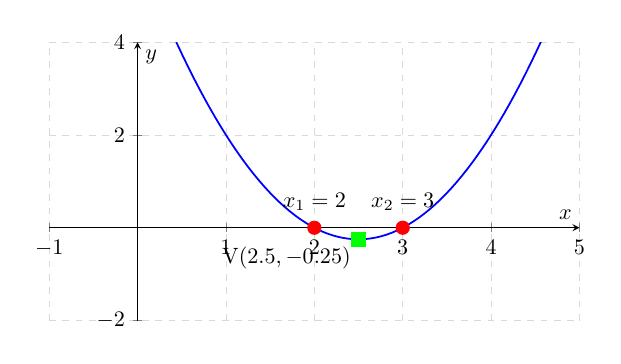
\begin{tikzpicture}[scale=0.8]
\begin{axis}[
    axis lines = center,
    xlabel = {$x$},
    ylabel = {$y$},
    ymin=-2, ymax=4,
    xmin=-1, xmax=5,
    grid=major,
    grid style={dashed,gray!30},
    width=10cm,
    height=6cm
]
% Parábola
\addplot[domain=-1:5, samples=100, thick, blue]{x^2-5*x+6};
% Raízes
\addplot[only marks, mark=*, mark size=3pt, red] coordinates {(2,0) (3,0)};
% Vértice
\addplot[only marks, mark=square*, mark size=3pt, green] coordinates {(2.5,-0.25)};
% Labels
\node[above] at (axis cs:2,0.2) {$x_1=2$};
\node[above] at (axis cs:3,0.2) {$x_2=3$};
\node[below left] at (axis cs:2.5,-0.25) {V$(2.5,-0.25)$};
\end{axis}
\end{tikzpicture}
\end{center}

\textbf{Interpretação geométrica final:}
As raízes $x_1 = 2$ e $x_2 = 3$ são os abcissas dos pontos de intersecção da parábola com o eixo dos xx. Geometricamente, representam os valores de $x$ para os quais a função $f(x) = x^2-5x+6$ se anula. A distância entre as raízes é $|x_2-x_1| = 1$, e o eixo de simetria da parábola passa pelo ponto médio entre elas, ou seja, em $x = 2.5$.
}